% !TEX root = ../main.tex

\chapter{系统安全性分析}


\section{原子性与可退款性分析}


跨链资产交换最重要的安全目标是原子性，即交换要么两侧都完成，要么双方都能够回到安全状态。本文系统通过两种路径实现这一目标，分别对应合约链的 HTLC 机制和无脚本链的 adaptor signature 机制。


\subsection{HTLC 路径的原子性}


在 HTLC 路径中，源链和目标链都使用相同 hashLock 创建锁定，两侧领取条件被同一个 secret 绑定。正常完成时，Bob 在目标链提交 secret 领取资产，secret 随之公开上链；源链参与方观察到 secret 后，可以用同一 secret 完成源链结算。失败时，secret 未公开，任何一方都无法领取资产，timeLock 到期后双方分别退款。


原子性的关键约束在于 timeLock 的不对称设置。目标链 ManagerB 的 timeLock 必须严格短于源链 Alice 的 timeLock。原因如下：Bob 需要在目标链 timeLock 到期前提交 secret 领取资产；secret 公开后，源链参与方需要在源链 timeLock 到期前使用该 secret 完成结算。如果两侧 timeLock 相同或目标链更长，则可能出现以下攻击场景——Bob 在目标链领取资产公开 secret，但源链 timeLock 已经到期，Alice 已经退款，导致 Bob 获得目标链资产的同时 Alice 也取回了源链资产，破坏原子性。因此，合理的设置应满足：timeLock\_source \textgreater{} timeLock\_target + 安全余量，其中安全余量需覆盖链上交易确认时间和参与方的响应延迟。


\subsection{Adaptor signature 路径的原子性}


在 adaptor signature 路径中，原子性由签名补全与秘密提取的密码学绑定保证。Alice 和 Bob 分别为各自链上的交易创建预签名，预签名与同一个秘密点 T = tG 绑定。当持有秘密 t 的一方补全签名并广播交易时，另一方可以从链上出现的有效签名与预签名的差值中提取 t，进而补全自己一侧的签名完成交易。


这一路径的原子性不依赖链上合约验证 secret，而依赖以下密码学保证：不知道 t 的一方无法补全预签名（不可伪造性）；一旦补全后的签名上链，t 必然可被提取（秘密提取必然性）。失败退出则通过预先签署的 timeLock 退款交易实现——如果在约定时间内没有任何一方广播补全后的签名，双方可以广播退款交易取回资产。与 HTLC 路径类似，退款交易的 timeLock 同样需要不对称设置，确保一方完成交易后另一方有足够时间提取秘密并完成己侧交易。


\subsection{原子性的前提假设}


两种路径的原子性都依赖以下前提：哈希函数和离散对数问题的计算安全性；链上交易能够在合理时间内被确认；参与方能够及时监听链上状态变化并在 timeLock 到期前做出响应。在这些前提下，系统能够保证跨链交换不会出现一方无条件获利而另一方无法退出的情况。


\section{针对Notary恶意行为的约束效果}


Notary 在系统中负责监听源链事件并协调目标链响应，是跨链流程的关键中间环节。本节通过分析 Notary 可能的恶意行为及系统的对应防御，明确其信任边界。


\subsection{Notary攻击和威胁分析}


假设 Notary 为理性攻击者，可能采取以下恶意行为：


拒绝服务：Notary 不转发源链事件，导致目标链 ManagerB 无法创建对应锁定，跨链流程停滞。系统防御：Alice 的源链资产受 timeLock 保护，到期后可无条件退款。Notary 的拒绝服务只影响可用性（交换无法完成），不影响资产安全性（Alice 不会损失资产）。


参数篡改：Notary 向目标链转发错误的 recipient、amount 或 hashLock。系统防御：如果 hashLock 被篡改，Bob 持有的 secret 无法匹配目标链锁定，交换无法完成，最终双方退款；如果 recipient 被篡改为攻击者地址，攻击者仍然需要正确 secret 才能领取，而 secret 由 Alice 生成并控制；如果 amount 被篡改为更小值，Bob 可以拒绝接受（链下协商层面），或者系统通过源链事件与目标链锁定的参数校验发现不一致。


重放攻击：Notary 对同一笔源链事件重复向目标链发起锁定请求。系统防御：合约要求同一 hashLock 不能重复创建 ManagerLock，重复请求会被拒绝。


抢跑攻击：Notary 观察到 secret 后抢先在目标链领取资产。系统防御：目标链 ManagerLock 的 recipient 字段限定了领取方，即使 Notary 知道 secret，也无法将资产转移到非指定地址。


\subsection{Notary 信任边界总结}


基于以上对notary可能发起的攻击的分析，可以看到，notary 的权力被限定为``消息传递和流程触发"，不具备绕过 hashLock 领取资产、修改合约状态或阻止退款的能力。其主要风险是可用性风险（拒绝服务导致交换失败）和协调正确性风险（参数错误导致流程异常），而非直接的资产盗取风险。后续可通过多 Notary 节点、多签触发或门限签名机制降低单点可用性风险。


\section{针对Manager约束效果分析}


Manager 负责资金池管理，持有或控制一定流动性，是系统中权限较高的角色。本节分析 Manager 可能的恶意行为及合约层面的约束机制。


\subsection{Manager攻击和威胁分析}


假设 Manager 为恶意参与方，可能采取以下行为：


拒绝响应：ManagerB 收到 Notary 的协调请求后拒绝创建目标链锁定。影响：跨链流程无法推进，但 Alice 的源链资产受 timeLock 保护，到期后可退款。Manager 的拒绝响应等价于 Notary 拒绝服务的效果，只影响可用性。


伪造锁定参数：ManagerB 创建锁定时使用错误的 recipient 或 amount。系统防御：如果 recipient 错误，真正的 Bob 无法领取，secret 不会被公开，最终双方退款；后端和前端可以通过比对源链事件与目标链锁定参数发现不一致，提醒用户不要公开 secret。


抢先领取：Manager 试图在 Bob 之前使用 secret 领取目标链资产。系统防御：completeManagerLock 函数将资产释放给 ManagerLock 中记录的 recipient 地址，而非调用者地址。即使 Manager 调用完成函数，资产仍然转给 Bob。


绕过 hashLock 直接释放：Manager 试图不经过 secret 验证直接转移锁定资产。系统防御：合约中资产释放逻辑要求 keccak256(secret) == hashLock 验证通过，且状态标记为 completed 后才执行转账。Manager 的 onlyManager 权限仅允许其创建锁定和超时退款，不能绕过完成条件。


密钥泄露：Manager 的私钥被第三方获取。影响：攻击者可以以 Manager 身份创建任意锁定或执行退款，但仍然无法绕过 hashLock 领取已锁定资产。主要风险是攻击者可以在 timeLock 到期前抢先退款，导致 Bob 无法领取。缓解措施包括多签管理、硬件密钥和限额控制。


\subsection{约束总结}


Manager 的行为受合约状态机约束：创建锁定需要指定完整参数且 hashLock 不可重复使用，完成交易需要正确 secret，退款需要 timeLock 到期且交易未完成。Manager 不能单方面绕过这些条件获取用户资产。其剩余风险主要在运营层面（流动性不足、响应延迟、密钥管理），可通过多签、限额和监控机制进一步缓解。


\section{异构链兼容性与安全等价性分析}


本文系统在合约链上使用 HTLC，在无脚本链场景使用 adaptor signature，两种机制在实现层不同但服务于相同的安全目标。本节分析两种机制在安全性保证上的等价性以及多机制兼容可能引入的风险。


\subsection{安全等价性}


HTLC 路径的安全性依赖：哈希函数的抗原像性（不知道 secret 无法通过 hashLock 验证）和 timeLock 的时间约束（到期前无法退款，到期后可无条件退款）。Adaptor signature 路径的安全性依赖：离散对数问题的困难性（不知道秘密 t 无法补全预签名）和预签署退款交易的时间约束（到期前退款交易无效，到期后可广播退款）。


两种机制在抽象层面提供相同的安全保证：完成条件绑定（一方完成交易必然导致秘密公开，使另一方具备完成条件）和失败安全退出（超时后双方可独立退款）。差异在于密码学假设不同——HTLC 依赖哈希函数安全性，adaptor signature 依赖椭圆曲线离散对数假设——但两者在当前计算能力下均被认为是安全的。


\subsection{跨机制秘密传递}


当跨链交换的两侧分别使用不同机制时（例如源链为 HTLC，目标链为 adaptor signature），需要确保秘密能够在两种机制之间正确传递。在本文系统中，HTLC 使用的 secret 与 adaptor signature 使用的秘密 t 可以建立对应关系：令 hashLock = H(secret) 且 T = tG，其中 secret 和 t 可以是同一个值或通过确定性派生关联。当 Bob 在 adaptor signature 侧补全签名广播交易后，Alice 从链上提取 t，即可作为 secret 在 HTLC 侧完成领取。这一跨机制传递的正确性依赖于 secret/t 的一致性约定，系统在初始化阶段需确保两侧使用的秘密值相互对应。


\subsection{多机制兼容的潜在风险}


多机制兼容引入的额外风险主要包括：时间窗口不匹配（两侧链的出块速度和确认时间不同，可能导致一侧 timeLock 到期时另一侧仍有未确认交易）；秘密格式不兼容（HTLC 的 secret 通常为 bytes32，adaptor signature 的 t 为椭圆曲线标量，需要确保编码和哈希方式一致）；监听延迟（从无脚本链上提取签名差值需要等待交易确认，期间源链 timeLock 持续消耗）。这些风险可以通过充分的 timeLock 安全余量、统一的秘密编码规范和及时的链上监听机制加以缓解。


\section{信任职责与资产职责的分离}


前面几节分析了系统在原子性、Notary 行为和 Manager 行为上的安全约束。本节从另一个角度讨论本文角色模型的一个结构性优势：将\textbf{信任职责}与\textbf{资产职责}分离开来，从而避免传统资金托管型方案中公证人角色固有的流动性问题。

\subsection{传统资金托管型方案的流动性枯竭}


在许多跨链桥和公证人方案中，公证人既是交易的信任协调方，又直接充当资金托管与做市方。以一个 ETH 到 Conflux 的转移为例：用户在源链将 ETH 交给公证人，公证人在目标链从自己的库存中取出等值 CFX 转给接收方。这种设计在单笔交换中看似自然，但在持续运行中会暴露出流动性单向枯竭的问题。

如果一段时间内的交换需求是单向的——例如大量用户都希望从 ETH 转移到 CFX——那么公证人的 ETH 库存只增不减，而 CFX 库存只减不增。最终公证人手中会积累大量 ETH，却耗尽了 CFX 库存。此时即使公证人持有的总价值很高，也无法再服务任何 ETH 到 CFX 的请求，因为目标链一侧已经无货可放。要维持服务，公证人必须不断进行跨链再平衡（rebalancing），将累积的 ETH 换回 CFX 并搬运回目标链库存，这本身又是一次有成本、有风险的跨链操作。

更进一步，这种模式抬高了参与门槛：任何人想要成为公证人或中继节点，都必须预先准备两条链上的启动库存，否则无法开展服务。这使得公证人角色天然倾向于中心化——只有资本充足的实体才能担任。

\subsection{本文的职责分离设计}


本文系统将上述被混在一起的两类职责拆分到不同角色上。Notary 只承担\textbf{信任职责}，即监听源链事件、转发跨链消息、推动目标链响应；它不接收用户在源链支付的资产，也不向目标链接收方放款。资产的锁定与释放完全由 Manager 资金池在合约约束下完成。

这一分离带来两个直接结果。第一，Notary 不持有任何跨链资产，因此根本不会经历\textquotedblleft 某一侧资产单向累积、另一侧单向枯竭\textquotedblright 的过程——它在协助交换前后的链上资产状态不发生变化，唯一的支出是自身发起目标链交易所消耗的 gas。运行一个 Notary 节点不需要任何启动库存，首个中继节点即可零资本接入。这与本章前述的信任边界分析相互印证：Notary 既偷不走资产（受 hashLock 与 timeLock 约束），也不需要为资产负责（不托管资产），其成本仅为在线时长与 gas，可由活跃窗口 $T_{\text{active}}$ 度量。

第二，流动性供给与再平衡的职责被清晰地隔离到 Manager 这一独立角色上。需要说明的是，职责分离并不意味着流动性枯竭问题被消除——如果交换长期单向，ManagerB 在目标链的资金池同样会被耗尽。本文的贡献不在于消除该问题，而在于把它从\textquotedblleft 与消息中继纠缠在一起\textquotedblright 的状态中剥离出来，使其成为一个边界明确、可独立监控和治理的问题。由于 Manager 是一个职责单一的角色，可以针对性地引入流动性监控、限额控制、动态费率和再平衡策略（参见第七章的展望），而不会影响 Notary 的轻量性和去中心化接入特性。

综上，本文角色模型在安全性之外提供了一个工程层面的结构性优势：通过将信任职责与资产职责分离，单点故障的性质从传统方案的\textquotedblleft 资本风险叠加可用性风险\textquotedblright 降低为 Notary 的\textquotedblleft 仅可用性风险\textquotedblright，同时大幅降低了中继节点的参与门槛。

\subsection{流动性枯竭的仿真验证}


为直观说明上述差异，本文对两种公证人模式在持续运行下的库存演化进行了仿真。仿真初始化 5 个传统资金托管型 notary，每个持有 ETH 与 CFX 各 10 单位；每一步随机选取一个 notary 参与一笔交换，方向为 ETH$\rightarrow$CFX 的概率为 $p$。一笔 ETH$\rightarrow$CFX 交换使该 notary 的 ETH 库存加一、CFX 库存减一（反向则相反），总量守恒；当某一币种库存不足时该方向无法服务，交换被拒绝。库存任一币种低于阈值（取 2）即视为流动性枯竭。作为对照，本文 Notary 不持有任何资产，库存恒定，仅累计 gas 开销。仿真共运行 2000 步。

图~\ref{fig:notary_unbiased} 给出无偏需求（$p=0.5$）的结果。左图以一个代表性 notary 为例展示其 ETH 与 CFX 库存的演化：每笔交换使一种币加一、另一种减一，库存随交换次数不断随机漂移，最终某一币种跌破阈值。即使两个方向的需求完全均衡，这种随机游走仍会使全部 5 个 notary 都触及枯竭阈值，平均首次枯竭出现在第 331 步，2000 笔交换中有 57 笔因库存不足被拒绝。这说明流动性枯竭并非单向需求所独有——随机性本身就足以使托管型 notary 的库存失衡。

\begin{figure}[htbp]
  \centering
  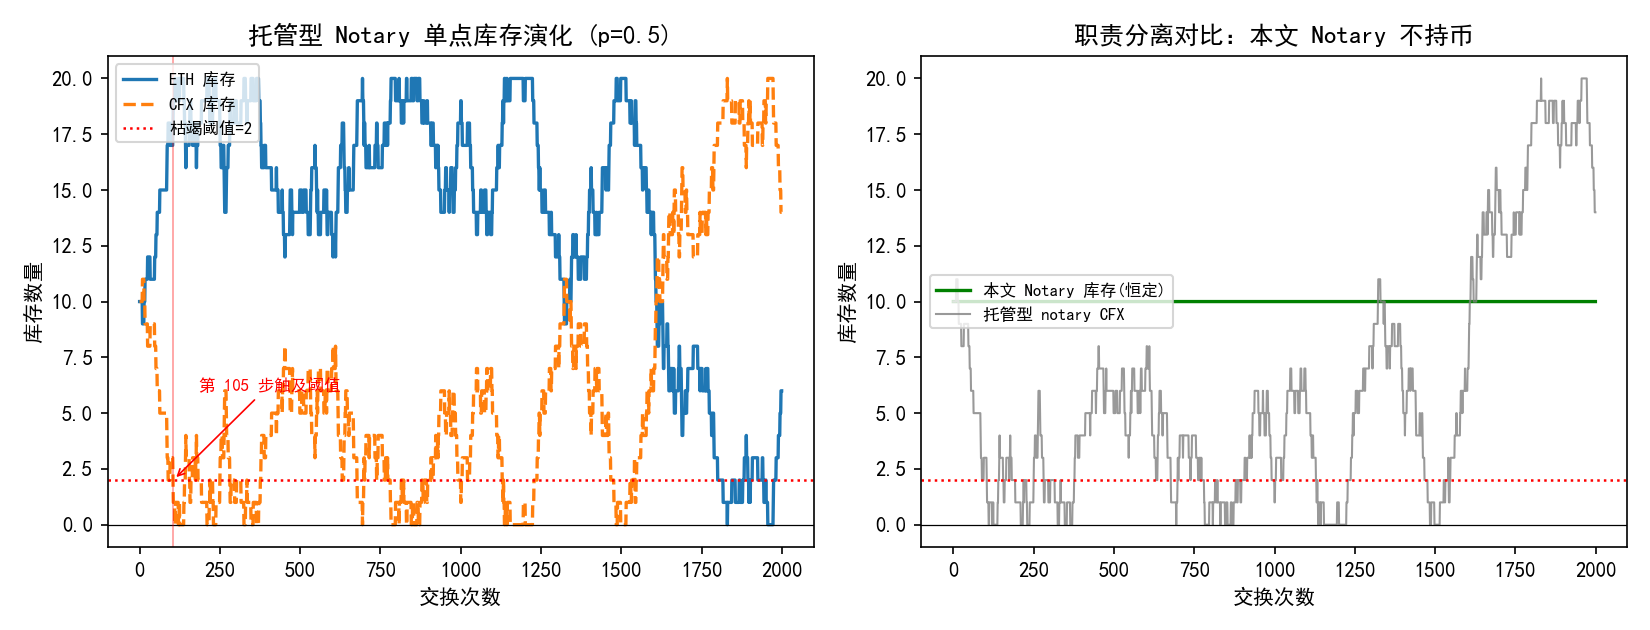
\includegraphics[width=0.95\textwidth]{figures/notary_liquidity_unbiased.png}
  \caption{无偏需求（$p=0.5$）下的库存演化。左图为一个代表性托管型 notary 的 ETH（实线）与 CFX（虚线）库存：每笔交换使一种币加一、另一种减一，库存随机漂移并在第 105 步触及阈值；右图将其与本文 Notary 的恒定库存对比}
  \label{fig:notary_unbiased}
\end{figure}

图~\ref{fig:notary_biased} 给出有偏需求（$p=0.7$，模拟单向跨链热点）的结果。左图同样以一个代表性 notary 展示：单向需求下其 CFX 库存被快速抽干、ETH 单向累积，第 80 步即触及阈值。从总体看枯竭显著加速，平均首次枯竭提前到第 106 步，末态各 notary 的 CFX 库存几乎归零而 ETH 大量累积，2000 笔交换中高达 809 笔（约 40\%）因目标链无货而被拒绝——这正对应\textquotedblleft 公证人最终只剩源链资产、却无法继续服务\textquotedblright 的失衡状态。与之相对，本文 Notary 在两种工况下库存始终恒定、拒绝交换数为零，不受流动性限制。

\begin{figure}[htbp]
  \centering
  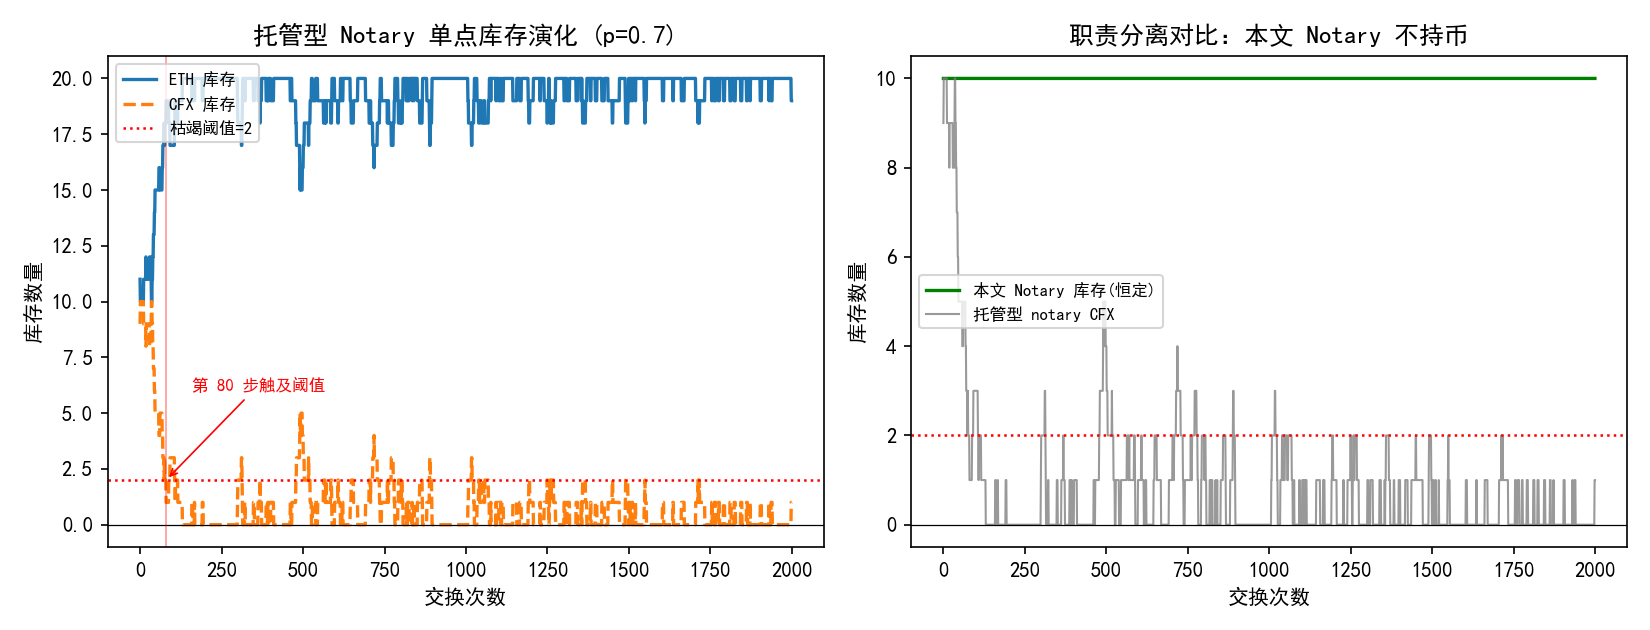
\includegraphics[width=0.95\textwidth]{figures/notary_liquidity_biased.png}
  \caption{有偏需求（$p=0.7$）下的库存演化。左图为一个代表性托管型 notary 的 ETH（实线）与 CFX（虚线）库存：单向需求下 CFX 快速耗尽、ETH 单向累积，第 80 步即触及阈值；右图与本文 Notary 的恒定库存对比}
  \label{fig:notary_biased}
\end{figure}

需要再次强调仿真的边界：该实验对象是 Notary 角色，结论为\textquotedblleft 托管型 notary 必然因库存失衡而枯竭，本文 Notary 因不持有资产而免疫\textquotedblright，并不代表本文系统整体不存在流动性问题——目标链 Manager 资金池在长期单向交换下同样会被耗尽。本文的价值在于将这一问题从消息中继职责中剥离，隔离到可独立治理的 Manager 角色，而非声称消除了它。
